\documentclass[border=10pt]{standalone}
\usepackage{tikz}\usepackage{amsmath}\usetikzlibrary{arrows.meta}
\begin{document}
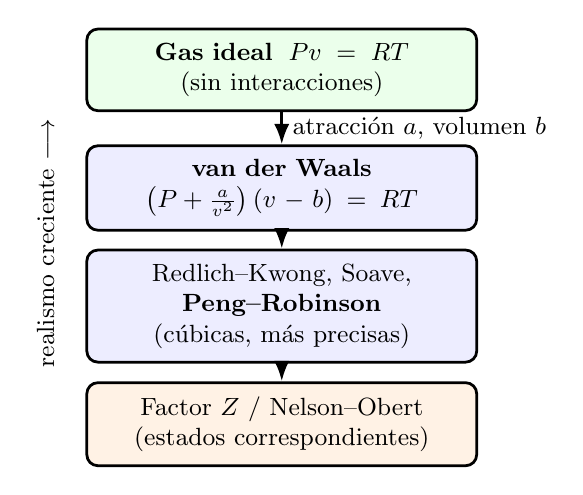
\begin{tikzpicture}[font=\small,>={Latex[length=2.6mm]},
  nd/.style={draw,line width=1pt,rounded corners,fill=blue!7,align=center,inner sep=5pt,text width=4.6cm}]
  \node[nd,fill=green!8] (gi) at (0,0) {\textbf{Gas ideal} \;$Pv=RT$\\(sin interacciones)};
  \node[nd] (vdw) at (0,-1.5) {\textbf{van der Waals} \;$\left(P+\frac{a}{v^2}\right)(v-b)=RT$};
  \node[nd] (rk) at (0,-3.0) {Redlich--Kwong, Soave, \textbf{Peng--Robinson}\\(cúbicas, más precisas)};
  \node[nd,fill=orange!10] (z) at (0,-4.5) {Factor $Z$ / Nelson--Obert\\(estados correspondientes)};
  \draw[->,line width=1.1pt] (gi)--(vdw) node[midway,right]{atracción $a$, volumen $b$};
  \draw[->,line width=1.1pt] (vdw)--(rk);
  \draw[->,line width=1.1pt] (rk)--(z);
  \node[rotate=90] at (-3.0,-2.2){\small realismo creciente $\longrightarrow$};
\end{tikzpicture}
\end{document}
